\documentclass[10pt,twocolumn,letterpaper]{article}

\usepackage{cvpr}
\usepackage{times}
\usepackage{epsfig}
\usepackage{graphicx}
\usepackage{amsmath}
\usepackage{amssymb}

% Include other packages here, before hyperref.

\usepackage{subfigure}

% If you comment hyperref and then uncomment it, you should delete
% egpaper.aux before re-running latex.  (Or just hit 'q' on the first latex
% run, let it finish, and you should be clear).
\usepackage[breaklinks=true,bookmarks=false]{hyperref}

\cvprfinalcopy % *** Uncomment this line for the final submission

\def\cvprPaperID{13} % *** Enter the CVPR Paper ID here
\def\httilde{\mbox{\tt\raisebox{-.5ex}{\symbol{126}}}}

% Pages are numbered in submission mode, and unnumbered in camera-ready
%\ifcvprfinal\pagestyle{empty}\fi
\setcounter{page}{1}
\begin{document}

%%%%%%%%% TITLE
\title{Fast Bird Part Localization for Fine-Grained Categorization}

\author{Yaser Souri\\
Sharif University of Technology\\
{\tt\small ysouri@ce.sharif.edu}
\and
Shohreh Kasaei\\
Sharif University of Technology\\
{\tt\small skasaei@sharif.edu}
}

\maketitle
%\thispagestyle{empty}

%%%%%%%%% ABSTRACT
%\begin{abstract}
%   Many recent papers in fine-grained categorization show the importance of part location information
%   for this task.
%   The state-of-the-art approach for part localization uses a convolutional neural network and needs
%   thousands of forward passes of the network which is very time consuming. An efficient method that needs only one forward pass for part localization is proposed. The method also provides
%   desirable properties such as improved generalization capability and the ability to detect multiple part 
%   instances simultaneously without much computational overhead. Experiments on Caltech-UCSD Birds
%   dataset show that the proposed method while being much faster achieves comparable accuracy to the
%   state-of-the-art method on this dataset.
%\end{abstract}

\begin{abstract}
Incorporating precise part information has proved to be crucial in building accurate fine-grained categorization systems in recent studies. The state-of-the-art approach for part localization uses a convolutional neural network and needs thousands of forward passes of the network, which is very time consuming. In this paper, an efficient method is proposed for part localization, with only one forward pass of the network. The proposed method provides improved generalization capability, compared to the state-of-the-art, and the ability to detect multiple part instances simultaneously, without much computational overhead. Experiments on the Caltech-UCSD Birds dataset show that the proposed method, while being much faster, achieves comparable accuracy to the state-of-the-art.
\end{abstract}

%%%%%%%%%%%%%%%%%%%%%%%%%%%%%%%%%%%%%%%
% 1
%%%%%%%%%%%%%%%%%%%%%%%%%%%%%%%%%%%%%%%
\section{Introduction}

Many recent papers on fine-grained categorization reveal the importance of accurate part location information. For instance, the methods proposed in \cite{poof} and \cite{partrcnn} are able to significantly boost their categorization performance using ground truth part locations at test time compared to when they estimate the part locations. Since the availability of part locations at test time is unrealistic, it is important to precisely localize parts automatically for build an accurate fine-grained categorization system.

The state-of-the-art method of PartRCNN \cite{partrcnn} uses the RCNN \cite{rcnn} approach for localizing parts. 
RCNN while producing excellent results for object detection, and in this case part localization, needs approximately 2000 forward passes of a typical {\it convolutional neural network} (CNN), which is very time consuming. This huge computational overhead makes PartRCNN unpractical for real-time and low power use cases (e.g., mobile devices). In this work, an efficient method that can be used for part localization (e.g., localizing a bird-head) is introduced. Compared to PartRCNN, our method has many desirable properties: (i) \textit{Computational complexity}. It only needs one forward pass of the same typical CNN, which makes it orders of magnitude faster than PartRCNN. (ii) \textit{Generalization}. This method can localize parts of objects from unseen classes, in difficult poses, and even on pictures of pencil drawings. It can also be trained to localize the bounding box of the whole object. (iii) \textit{Multiple part localization}. This method is able  to localize multiple part instances without much computational overhead (still using only one forward pass of the CNN).

%%%%%%%%%%%%%%%%%%%%%%%%%%%%%%%%%%%%%%%
% 2
%%%%%%%%%%%%%%%%%%%%%%%%%%%%%%%%%%%%%%%
\section{Proposed Method}
We cast the problem of bird part localization as classifying pixels of the image to whether each pixel belongs to the part (positive) or not (negative). To this end, a feature vector for each pixel and a classifier for each part is needed. The convolutional layers of AlexNet \cite{alexnet} network pretrained on ILSVRC dataset \cite{ilsvrc} is used to extract the feature vectors. First, the input image is resized to the input dimension of AlexNet (i.e., 227x227). Then, with a single forward pass, the convolutional feature maps (\textit{conv1}-\textit{conv5}) for the input image is computed. Each feature map is then up-sampled to 227x227 as shown in Figure \ref{fig:method}.

\begin{figure}
	\centering
	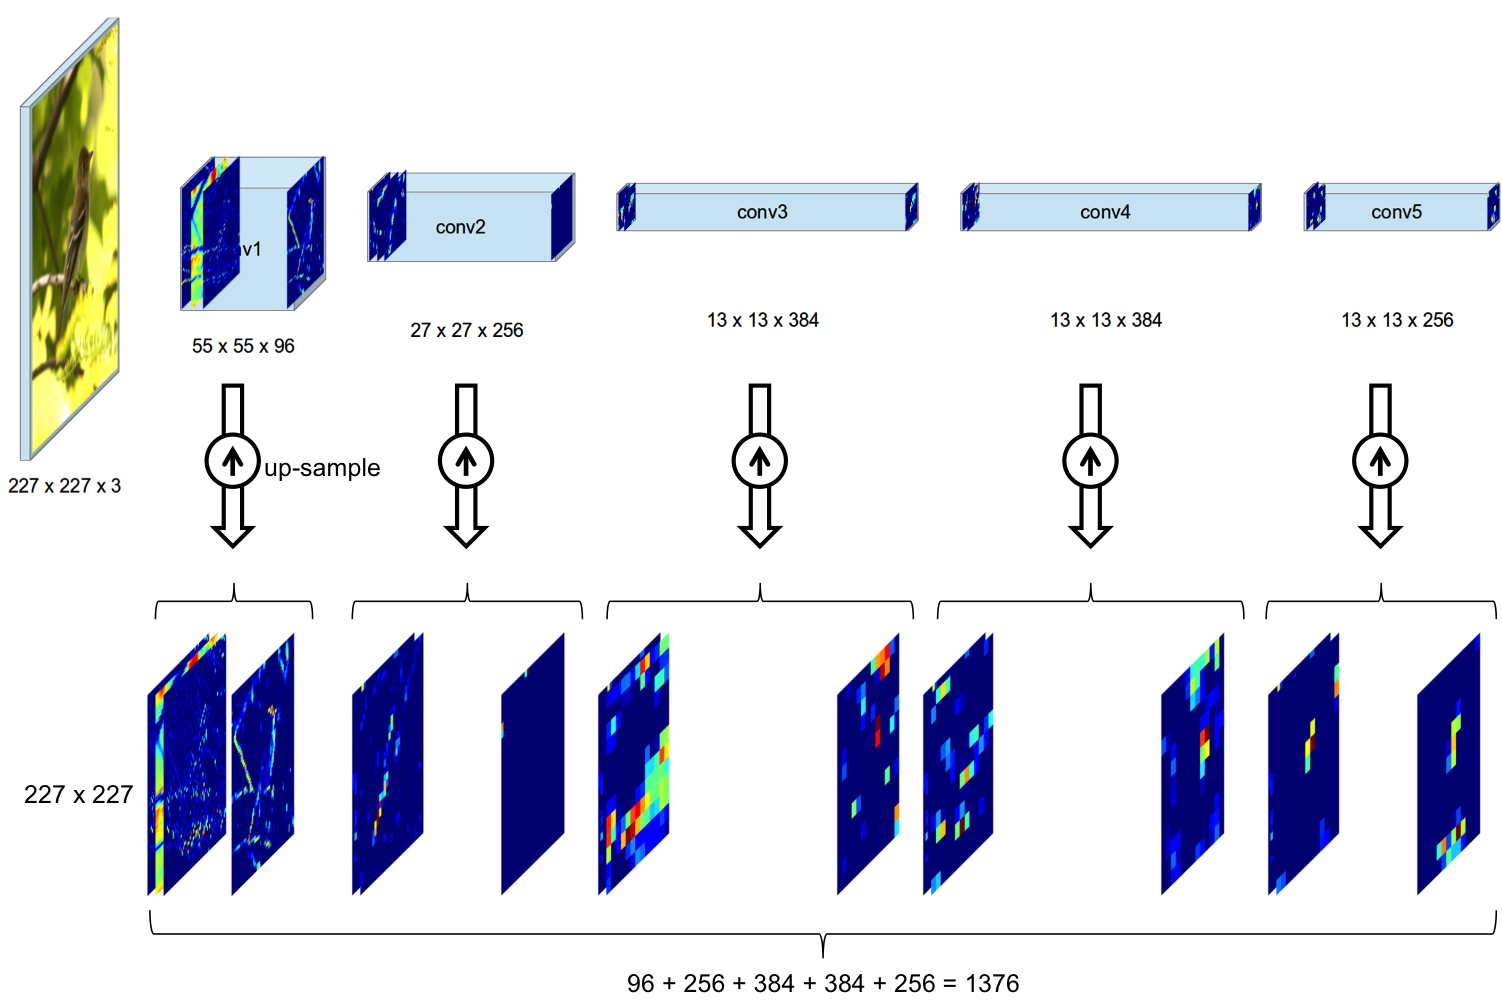
\includegraphics[height=6cm]{images/deeprf}
	\caption{Overview of feature extraction step using the AlexNet \cite{alexnet} architecture. Input image is resized to a fixed dimension. CNN computes the feature maps in convolutional layers. Each feature map is then up-sampled to the fixed input dimension.}
	\label{fig:method}
\end{figure}

\begin{figure*}
	\centering
	\subfigure[]{
		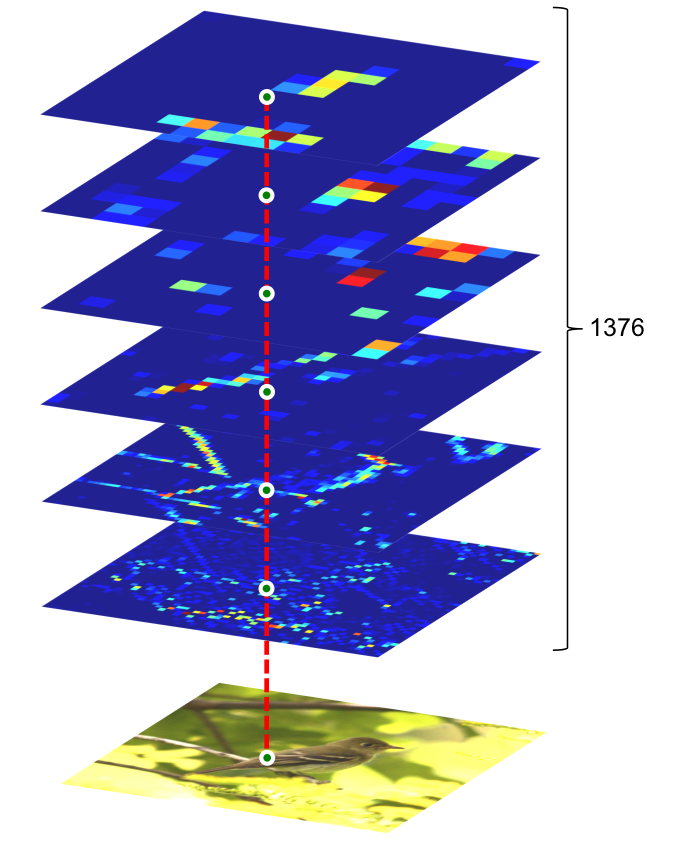
\includegraphics[height=3cm]{images/hypercolumn}
		\label{fig:hyper}
	}
	\subfigure[]{
		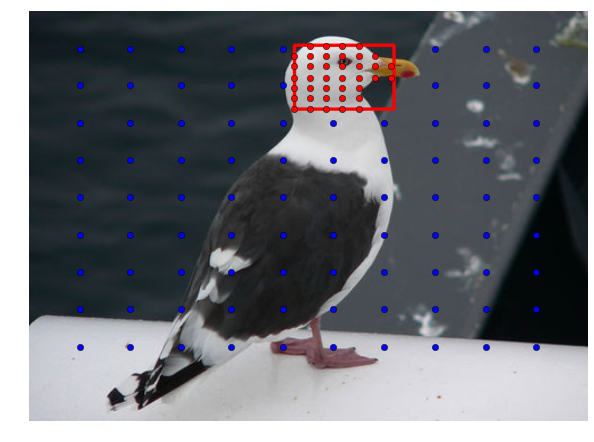
\includegraphics[height=3cm]{images/training_points}
		\label{fig:points}
	}
	\subfigure[]{
		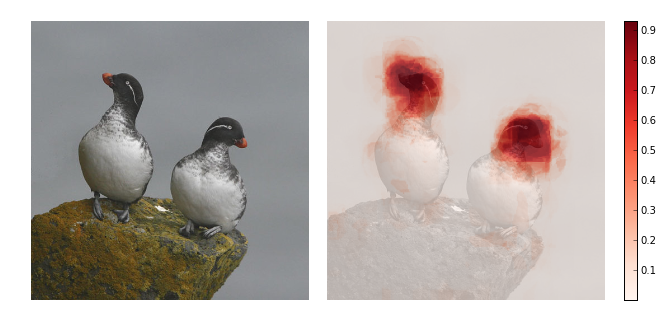
\includegraphics[height=3cm]{images/re_multiple}
		\label{fig:r_m}
	}
	\subfigure[]{
		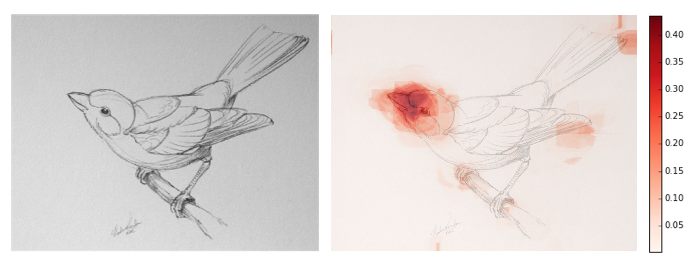
\includegraphics[height=3cm]{images/re_drawing}
		\label{fig:r_d}
	}
	\subfigure[]{
		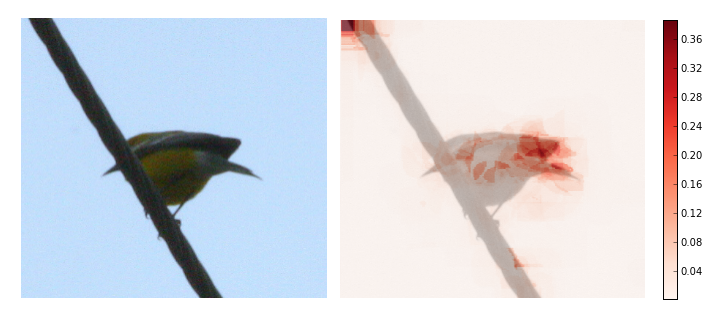
\includegraphics[height=3cm]{images/re_nohead}
		\label{fig:r_n}
	}
	\caption{
\subref{fig:hyper} Feature vector for each pixel is extracted from up-sampled feature maps. \subref{fig:points} A set of positive (red) and negative (blue) points used for training a bird-head localizer.
In \subref{fig:r_m}, \subref{fig:r_d}, and \subref{fig:r_n} on the left is the input image and on the right is the estimated probability of presence of bird's head-part in each pixel (in red). Colorbar shows the actual probability value estimated for the corresponding image.
}
	\label{fig:results}
\end{figure*}

For AlexNet architecture, this gives a total of 1376 feature maps. The feature maps are stacked to form a hypercolumn (inspired by \cite{hypercolumn}). For each pixel in position $(x,y)$ in the image, a 1376 dimensional feature vector is extracted from this hypercolumn by concatenating filter response values at position $(x,y)$ from all feature maps (Figure \ref{fig:hyper}).

We use a {\it Random Forest} classifier due to its many desirable properties \cite{rf_book} including but not limited to its speed and its ability to produce probability estimates. For training the classifier, the training set of CUB \cite{cub} dataset is used to create two pools of positive and negative pixels with their corresponding pixel-wise deep features. For each image, first the hypercolumn is created with a forward pass of the CNN. Then, a set of 20 positive pixels, uniformly spaced, which are located inside the bounding box of the part (e.g., bird-head) are added to the positive pool of pixels with their corresponding feature values. The same is done for 40 negative points which are not located inside the part bounding box (Figure \ref{fig:points} shows these points for an image). Then, the Random Forest is trained to classify positive and negative points discriminatively. At test time, all pixels are (densely) classified using the trained Random Forest resulting in a single channel image where each pixel's value is the probability of that pixel belonging to the part (see Figures \ref{fig:r_m}-\subref{fig:r_n}.) This method can detect multiple parts simultaneously (Figure \ref{fig:r_m}); detect head of birds in pencil drawings (Figure \ref{fig:r_d}) and also detect situations where the head is not clearly visible (Figure \ref{fig:r_n}) with low probabilities.

%%%%%%%%%%%%%%%%%%%%%%%%%%%%%%%%%%%%%%%
% 3
%%%%%%%%%%%%%%%%%%%%%%%%%%%%%%%%%%%%%%%
\textbf{Classification Pipeline:}
A similar pipeline as PartRCNN \cite{partrcnn} is used for classification.
A part bounding box is obtained from each probability estimate of part location (produced by our method) by thresholding and selecting the enclosing rectangle of the largest connected component.
%From each probability estimate of part location produced by our method, a bounding box is obtained by thresholding and selecting the enclosing rectangle of the largest connected component.
Three Random Forests are trained to localize the bird's bounding box, head, and body. Furthermore, for feature extraction (fc7 layer), four different AlexNet networks are fine-tuned (namely, the entire image and the bird's bounding box, body, and head). 
A linear SVM is used for categorization. With this setup, the method achieves $72.35\%$ mean accuracy for categorization, which is comparable to PartRCNN \cite{partrcnn} ($73.89\%$), while being at least 2 orders of magnitude faster.

\textbf{Acknowledgments:}
We would like to thank Dr. Ehsan Adeli for his help in writing the paper.

{\scriptsize
\bibliographystyle{ieee}
\bibliography{egbib}
}

\end{document}